\documentclass[10pt,a4paper]{article}
\usepackage[margin=1.8cm]{geometry}
\usepackage[T1]{fontenc}
\usepackage[utf8]{inputenc}
\usepackage{lmodern,microtype,amsmath,amssymb,booktabs,graphicx,float}
\usepackage{caption}
\usepackage[hidelinks]{hyperref}
\usepackage{enumitem}
\IfFileExists{libertine.sty}{\usepackage{libertine}}{}
\IfFileExists{inconsolata.sty}{\usepackage{inconsolata}}{}

\graphicspath{{figures/}}
\setlength{\parindent}{0pt}
\setlength{\parskip}{5pt}
\captionsetup{font=small,labelfont=bf}
\setlist{nosep,leftmargin=*}
\newcommand{\Rtwo}{R\textsuperscript{2}-Gaussian}
\title{\vspace{-1.3cm}\large\bfseries TRDP2: Limited-Angle 3D CT Reconstruction with \Rtwo\\[4pt]
\normalsize Week 3: Ordinary-TV Controls and Generalization Preparation}
\author{\normalsize Md Zunayedul Islam \qquad Biswarup Mukherjee}
\date{\small Weekly Progress Report: 3--9 October 2026\\Evidence cutoff: 8 October 2026}
\begin{document}
\maketitle
\vspace{-1em}
\begin{abstract}
This week extended the completed limited-angle pilot into a reproducible development benchmark and tested whether tuning ordinary total variation (TV) could reduce its reconstruction deficit. We reproduced the two 120$^\circ$ acquisitions and evaluated TV weights 0.025, 0.05, and 0.1 with paired input data, initializer bytes, seed, and iteration budget within each acquisition. The original weight 0.05 achieved the highest volume PSNR and slice-averaged SSIM at both orientations: 30.913/28.591 dB and 0.9010/0.8624 for acquisition starts 0$^\circ$/90$^\circ$. Lower TV slightly improved boundary errors but reduced SSIM; higher TV worsened both. The predeclared selection rule therefore retained 0.05. The 2.32 dB orientation gap remained. We also recorded a six-subject LIDC-IDRI candidate cohort and downloaded and audited the first development series. Independent-volume reconstruction has not yet been performed. Geometry-dependent regularization remains a hypothesis whose effectiveness and novelty are unverified.
\end{abstract}

\section{Objective and scope}
The previous report established that limiting angular coverage degrades reconstruction and that rotating a 120$^\circ$ acquisition changes its error pattern. This week focused on controls and reproducibility before introducing a new regularizer. Three questions guided the work:
\begin{enumerate}
\item Can the limited-angle baseline be reproduced through a guarded, auditable workflow?
\item Does changing the strength of ordinary TV improve both whole-volume accuracy and boundary preservation across the two development orientations?
\item What data and preprocessing checks are needed for an independent-volume evaluation with frozen settings?
\end{enumerate}
The primary objective is reconstruction generalization across acquisitions and independent volumes. Each scan still receives its own Gaussian optimization; no population-trained model was introduced. The reliability question raised in the previous report remains relevant, but no missing-view reliability predictor, uncertainty estimator, or geometry-conditioned penalty was implemented this week. Reference-derived errors are evaluation diagnostics, not inference-time uncertainty estimates.

\section{Dataset and experimental methods}
\subsection{Development data and acquisition pairing}
We retained the supplied \texttt{0\_chest\_cone} reference from \Rtwo\ \cite{r2,upstream}: a $256^3$ array in supplied normalized intensity units, not calibrated HU. Measurements were generated with TIGRE using the existing physical-geometry and detector-orientation conventions \cite{tigre}. Both development cases used 50 noise-free views, identical scanner geometry, and a 120$^\circ$ span:
\begin{equation}
\theta_i=\theta_{\mathrm{start}}+i\frac{120^\circ}{50},\quad i=0,\ldots,49,\qquad
\theta_{\mathrm{start}}\in\{0^\circ,90^\circ\}.
\end{equation}
The baseline was rerun through the new workflow; the historical pilot was preserved. The new common evaluation grid is
\begin{equation}
\phi_k=(k+0.25)\,3.6^\circ,\quad k=0,\ldots,99.
\end{equation}
The previous pilot used a 0.5-bin offset. That grid overlaps a proposed 90$^\circ$-span training grid, so the new benchmark uses a shared 0.25-bin offset, disjoint from all six planned acquisition grids. Both current 120$^\circ$ cases have 34 inside-arc and 66 outside-arc evaluation directions, compared with the pilot's 33/67. Historical projection metrics must therefore not be pooled with the new grid. Reference and evaluation arrays are copied byte-for-byte across paired acquisitions and verified by hashes.

\subsection{Reconstruction and ordinary-TV controls}
We retained the original \Rtwo\ training implementation and its existing data loss, density control, and TV definition. Each acquisition received its own FDK initializer \cite{fdk}: 50,000 points, sampling threshold 0.05, and density rescaling 0.15. Within an acquisition, all TV weights used the \emph{same saved initializer bytes}, training data, optimization seed zero, and 30,000 iterations. Between acquisitions, the FDK initializers differ because the measurements differ. Orientation sensitivity consequently includes initialization effects as well as optimization and measurement geometry.

The implemented loss retains its existing weighting conventions:
\begin{equation}
\mathcal L=\mathcal L_1+
\lambda_{\mathrm{DSSIM}}\mathcal L_{\mathrm{DSSIM}}+
\lambda_{\mathrm{TV}}\mathcal L_{\mathrm{TV}},\qquad
\lambda_{\mathrm{DSSIM}}=0.25.
\end{equation}
Ordinary TV is evaluated on the existing $32^3$ query patch. Its axiswise absolute differences are not normalized by physical voxel spacing; the code and definition were unchanged. We tested the predeclared grid $\lambda_{\mathrm{TV}}\in\{0.025,0.05,0.1\}$. The two completed 0.05 runs were reused, requiring four additional completed controls. Evaluation used the fixed final iteration, not a best checkpoint selected with the reference.

Before observing the controls, we recorded the following selection rule: a non-default weight is eligible only if \emph{neither} development orientation has worse boundary MAE or SSIM than its 0.05 baseline. Among eligible weights, choose the highest mean final volume PSNR across the two orientations; ties within 0.01 dB favor the default if present. This is a conservative development criterion, not a significance test.

\subsection{Evaluation and correctness checks}
Whole-volume metrics retain predictions without clipping or per-volume normalization. For the unit-range reference, with $N$ voxels,
\begin{equation}
\operatorname{MAE}=N^{-1}\sum_i|\hat x_i-x_i|,\quad
\operatorname{RMSE}=\sqrt{N^{-1}\sum_i(\hat x_i-x_i)^2},\quad
\operatorname{PSNR}=10\log_{10}(1/\operatorname{MSE}).
\end{equation}
SSIM is the inherited average of slice-wise scores over the three array axes \cite{ssim}; it is not a volumetric-window SSIM. All 256 slices were valid on each axis for the development reference.

We added a fixed reference-derived boundary diagnostic. On the common forward-difference interior, compute $\nabla_h x$ using supplied voxel spacings. Let $\tau$ be the 90th percentile of strictly positive gradient magnitudes, and define
\begin{equation}
B=\{i:\|\nabla_h x_i\|_2\geq\tau\},\quad
E_B=|B|^{-1}\sum_{i\in B}|\hat x_i-x_i|,\quad
G_B=|B|^{-1}\sum_{i\in B}\|\nabla_h\hat x_i-\nabla_h x_i\|_2.
\end{equation}
Ties are included. This mask contains 1,480,749 interior voxels and is identical across all six reconstructions. It is an operational high-gradient mask, not anatomical segmentation. Gradient units follow the supplied geometry, whose physical calibration is unknown.

The workflow checks manifest identity, source hashes, angle arrays, dataset file sets, initializer hashes, finite arrays, subprocess exit codes, and expected final artifacts. Existing destinations are rejected. A GPU smoke test isolates Gaussian query/gradient and TIGRE projection checks in separate processes: the forward projector's CUDA-context reset had caused a segmentation fault when combined with live PyTorch tensors. The isolated wrapped/unwrapped projection discrepancy was $1.71\times10^{-6}$ against a $10^{-5}$ tolerance. This verifies implementation consistency, not independent scanner physics.

\section{Results and interpretation}
\subsection{Reproduced baselines and TV selection}
The new default-TV baselines achieved 30.913 and 28.591 dB. The corresponding historical pilot values were approximately 30.907 and 28.594 dB. This close agreement supports workflow consistency; the small differences are not method improvements. No new full-circle run was needed for this control study.

\begin{table}[H]
\centering\small
\caption{Fixed-final volume results. Bold PSNR/SSIM identify the best value within each acquisition. All values come from verified completed runs; interrupted attempts are excluded.}
\begin{tabular}{ccrrrrr}
\toprule
Start & TV weight & PSNR (dB) & SSIM & MAE & RMSE & Boundary MAE\\
\midrule
0$^\circ$ & 0.025 & 30.766 & 0.8986 & 0.01408 & 0.02895 & 0.03833\\
0$^\circ$ & 0.05 & \textbf{30.913} & \textbf{0.9010} & 0.01370 & 0.02847 & 0.03880\\
0$^\circ$ & 0.1 & 30.782 & 0.8989 & 0.01395 & 0.02890 & 0.04060\\
\midrule
90$^\circ$ & 0.025 & 28.538 & 0.8602 & 0.01760 & 0.03742 & 0.05611\\
90$^\circ$ & 0.05 & \textbf{28.591} & \textbf{0.8624} & 0.01725 & 0.03719 & 0.05654\\
90$^\circ$ & 0.1 & 28.448 & 0.8602 & 0.01755 & 0.03781 & 0.05823\\
\bottomrule
\end{tabular}
\end{table}

Mean PSNR across orientations was 29.652, 29.752, and 29.615 dB for TV 0.025, 0.05, and 0.1, respectively. The original weight 0.05 was the only eligible choice under the recorded rule. Lower TV reduced boundary MAE by approximately 1.2\% and 0.7\%, but lowered SSIM at both orientations. Higher TV increased boundary MAE by approximately 4.6\% and 3.0\%, and reduced both PSNR and SSIM. Therefore, \textbf{0.05 is frozen as the ordinary-TV reference} for the next stage.

\begin{figure}[H]
\centering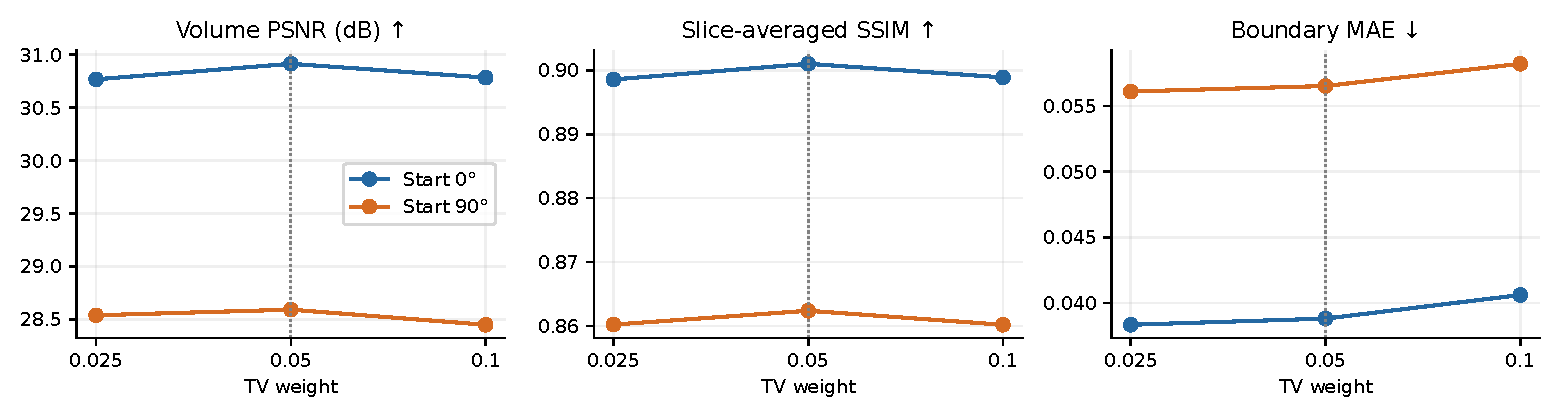
\includegraphics[width=\linewidth]{tv_tradeoff.pdf}
\caption{The three-weight development comparison. The dotted line marks the retained weight 0.05. Lower TV modestly improves the boundary metric while worsening global structure/accuracy. Higher TV offers no improvement in these metrics. Two orientations of one volume are paired development cases, not independent subjects.}
\end{figure}

\subsection{Residual orientation sensitivity and spatial errors}
At the selected weight, rotating the acquisition reduced PSNR by 2.321 dB, increased RMSE by about 31\%, and increased boundary MAE by about 46\%. This corresponds to approximately 1.71 times the voxel MSE. The gap remains under all three TV weights; this small scalar-weight search does not explain away the acquisition dependence observed in the pilot.

\begin{figure}[H]
\centering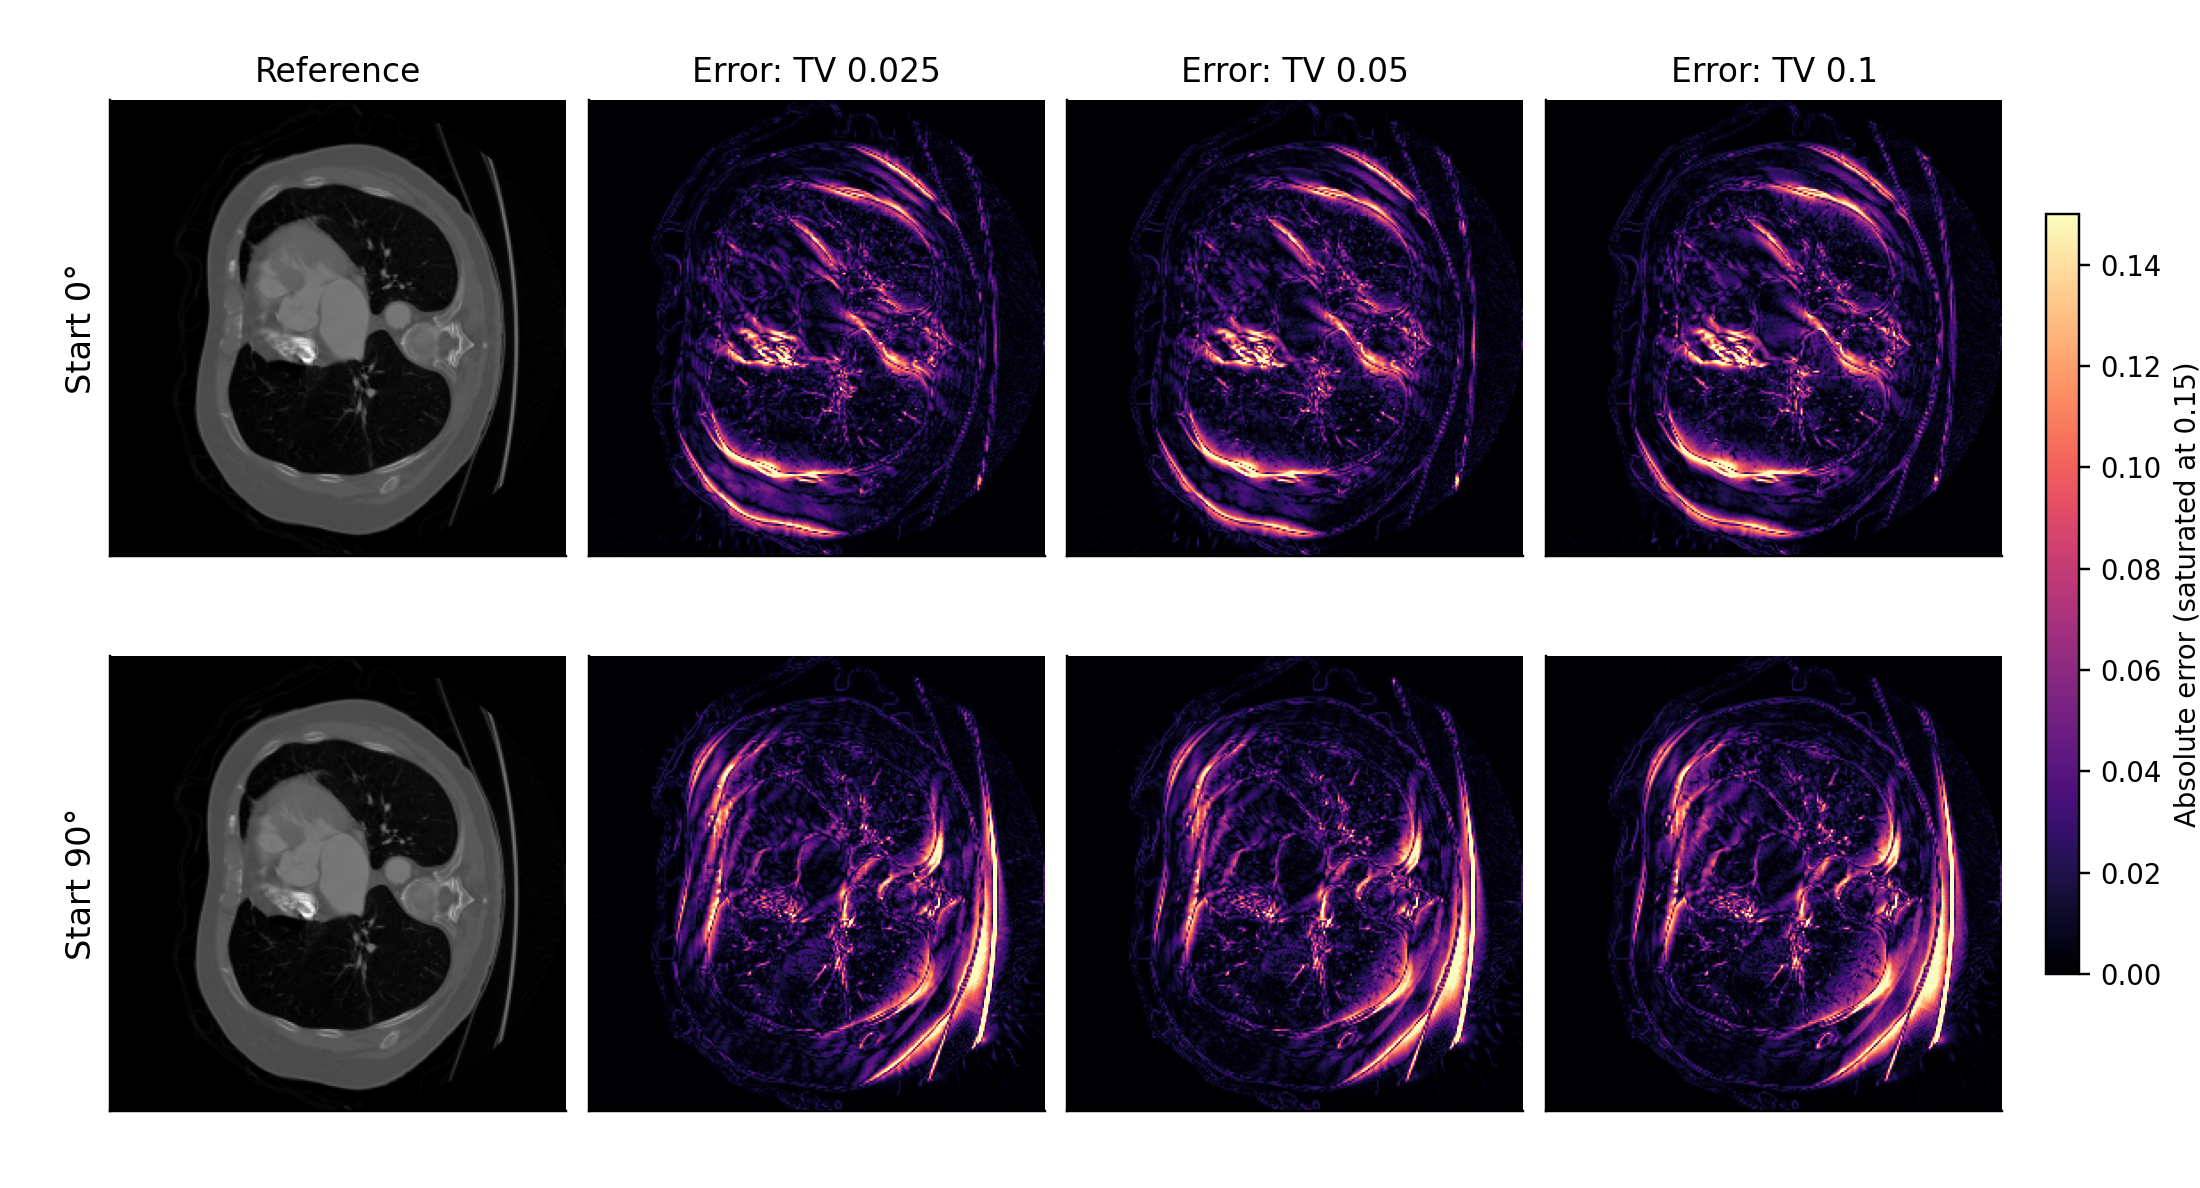
\includegraphics[width=.94\linewidth]{slice_errors.png}
\caption{Identical reference slice (array axis 2, index 128) and absolute errors for all TV weights at each orientation. Reference display window: [0,1]; all error panels: [0,0.15], with larger errors saturated. Only display values are saturated; numerical metrics are unclipped. The rotated case retains stronger structured boundary errors. This is a fixed central slice, not an optimized or anatomically selected example.}
\end{figure}

The boundary-gradient error $G_B$ at start 0$^\circ$ was 7.821, 7.990, and 8.418 for increasing TV weights; at start 90$^\circ$ it was 10.546, 10.703, and 11.056. These diagnostics agree that reducing ordinary TV can preserve some gradients, yet this does not translate into better whole-volume PSNR or SSIM. They do not show which geometry-dependent penalty direction, if any, would improve reconstruction.

\subsection{Optimization progress and projection diagnostics}
\begin{figure}[H]
\centering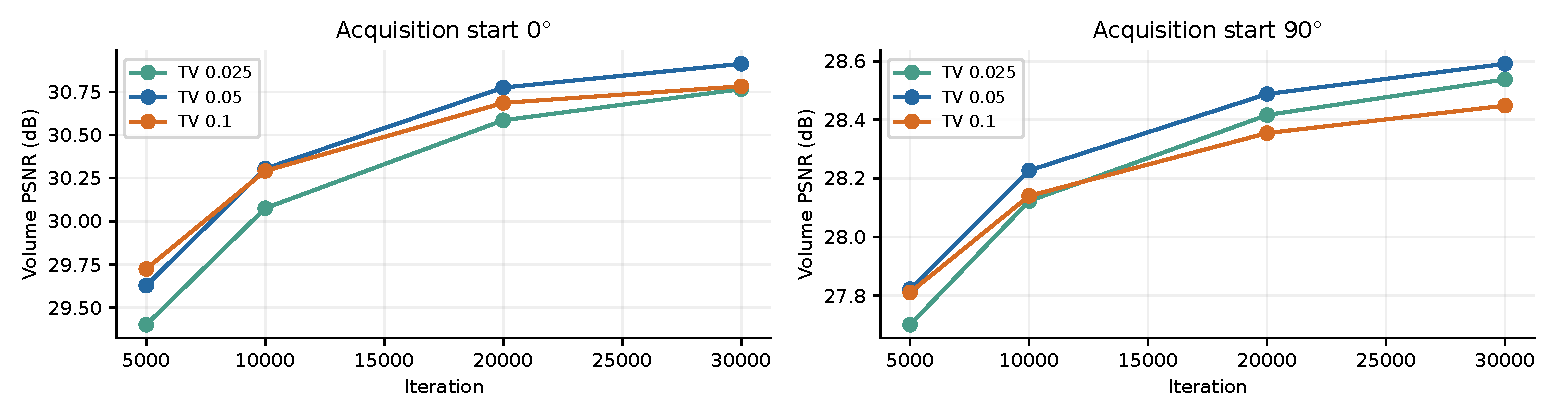
\includegraphics[width=\linewidth]{convergence.pdf}
\caption{Saved volume PSNR evaluations from iteration 5,000 onward. Curves are shown at the logged evaluation iterations without smoothing. Final selection always uses iteration 30,000. Diminishing gains at later iterations provide no evidence that simply extending these runs would close the orientation gap.}
\end{figure}

For the default-TV baselines, saved Gaussian-renderer evaluations gave mean inside/outside held-out PSNR of 51.49/39.81 dB at start 0$^\circ$ and 51.87/38.51 dB at start 90$^\circ$. Both use 34 inside and 66 outside directions. These are means of per-view PSNR, with each projection independently divided by its own maximum by the inherited projection metric. They are distinct from the unnormalized voxel-volume TIGRE MAE curves in the previous report. No new independent TIGRE reprojection comparison was completed for the TV grid. Strong agreement near measured angles alone is insufficient evidence of accurate volume reconstruction.

\subsection{Independent-volume intake}
Official NBIA metadata was retrieved for LIDC-IDRI subjects 0002--0007 \cite{lidc,nbia}. A provisional cohort was assigned before reconstruction: 0002--0003 for development/intake, 0004--0005 for validation, and 0006--0007 as final-test candidates. Selection follows ascending identifiers after excluding 0001; this is a small convenience cohort, not representative sampling. Each returned subject has one selected CT series, and metadata snapshots retain subject, study/series identifiers, license, collection DOI, and checksums.

The inherited raw-data configuration maps \texttt{0\_chest} to LIDC-IDRI-0001. This is a provenance lead rather than proof that the supplied array derives from that scan. Subject 0001 is excluded, while independence from the actual pilot remains unverified pending source reproduction or equivalent evidence.

Only development subject 0002 has been downloaded: a 67.4 MB ZIP containing 261 CT slices of $512\times512$ pixels, with spacing $0.681641\times0.681641\times1.25$ mm. Archive CRC, unique instance identifiers, subject/study/series identity, direction cosines, and slice-position consistency passed the header audit. Pixels have not been decoded for preprocessing validation, and no independent-volume reconstruction has run. The included license and provenance are retained; the LIDC-IDRI collection lists CC BY 3.0 \cite{lidc}.

\section{Limitations and next steps}
The completed quantitative study still uses one reference volume, one angular span, two orientations, noiseless synthetic data, one seed, and three TV strengths. It establishes a development reference, not statistical superiority or population transfer. Correlated slices and views are not independent experimental subjects. Jobs ran on multiple university workstations with the same GPU model; runtime and contention were uncontrolled, and peak VRAM was not measured. No speed comparison is supported.

Preprocessing is a central remaining issue. The inherited DICOM recipe sorts filenames, reverses slice order, clips intensities, applies per-volume min/max normalization, and resizes directly to a cube. Independent-volume testing requires audited physical ordering, orientation, spacing, padding, and a fixed intensity/FOV policy. Otherwise the same numerical TV weight may correspond to a different effective regularization strength. A fixed HU-window mapping is a candidate preprocessing choice, not a validated attenuation model.

Next steps are to:
\begin{enumerate}
\item Resolve the pilot's source identity and validate pixel decoding and physical-coordinate preprocessing on development subjects only.
\item Freeze intensity scaling, resampling, crop/FOV, and scanner-unit conventions before processing validation/final subjects.
\item Evaluate the frozen ordinary-TV reference on independent volumes at familiar geometry, then examine combined volume/acquisition shift. Keep the reserved acquisition results unexposed until their protocol is frozen.
\item Test any proposed geometry descriptor against operator perturbation responses before defining penalty direction or strength. Compare with ordinary TV, an equally tuned uniform penalty, and a deliberately wrong-orientation control.
\end{enumerate}
Geometry-dependent regularization remains a research hypothesis. This week's evidence neither demonstrates its benefit nor verifies novelty relative to existing geometry-conditioned reconstruction methods.

\section{Status and reproducibility}
The working research repository is \url{https://github.com/zunaaaaayed/trdp2}; the original method remains credited to \Rtwo\ \cite{r2,upstream}. At the evidence cutoff, commit \texttt{ba3e2b8} records fresh-attempt support, frozen TV results, candidate-cohort metadata, header auditing, and tests. The two relevant control/intake test suites passed 10 tests. Earlier backend, manifest, and baseline checks are retained in their respective records.

All six reported reconstructions use the fixed final iteration. Two interrupted TV 0.1 attempts are preserved but excluded from analysis. The accepted start-0$^\circ$ TV 0.1 run completed on \texttt{cheonech}; the accepted start-90$^\circ$ run is explicitly named \texttt{\_\_chani\_20261008}. Restarts use original initializer bytes and full iteration budgets, not unverified checkpoint continuation. The completed jobs include final checkpoints, finite volume checks, process completion records, and hashes. The final accepted job completed on 8 October at 13:55 Paris time.

Small results and protocols are versioned; raw images, checkpoints, and full logs remain on university storage. The earlier 7 October transfer archive predates these completed controls and is not a complete backup of the current state. Report figures are generated from the saved metrics and completed volumes by the accompanying \texttt{make\_figures.py}. No GPU experiment is needed to compile this report on Overleaf.

\begin{thebibliography}{9}\small
\bibitem{r2} R. Zha, T. J. Lin, Y. Cai, J. Cao, Y. Zhang, and H. Li. R$^2$-Gaussian: Rectifying Radiative Gaussian Splatting for Tomographic Reconstruction. \emph{NeurIPS}, 2024. \url{https://arxiv.org/abs/2405.20693}.
\bibitem{upstream} R. Zha et al. R$^2$-Gaussian: original implementation and dataset distribution. \url{https://github.com/Ruyi-Zha/r2_gaussian}.
\bibitem{tigre} A. Biguri, M. Dosanjh, S. Hancock, and M. Soleimani. TIGRE: A MATLAB-GPU toolbox for CBCT image reconstruction. \emph{Biomedical Physics \& Engineering Express}, 2(5):055010, 2016. \url{https://doi.org/10.1088/2057-1976/2/5/055010}.
\bibitem{fdk} L. A. Feldkamp, L. C. Davis, and J. W. Kress. Practical cone-beam algorithm. \emph{JOSA A}, 1(6):612--619, 1984. \url{https://doi.org/10.1364/JOSAA.1.000612}.
\bibitem{ssim} Z. Wang, A. C. Bovik, H. R. Sheikh, and E. P. Simoncelli. Image quality assessment: From error visibility to structural similarity. \emph{IEEE Transactions on Image Processing}, 13(4):600--612, 2004. \url{https://doi.org/10.1109/TIP.2003.819861}.
\bibitem{lidc} S. G. Armato III et al. Data from LIDC-IDRI. The Cancer Imaging Archive, 2015. \url{https://doi.org/10.7937/K9/TCIA.2015.LO9QL9SX}. Collection and usage terms: \url{https://www.cancerimagingarchive.net/collection/lidc-idri/}.
\bibitem{nbia} The Cancer Imaging Archive. NBIA Search REST API Guide. Accessed 8 October 2026. \url{https://wiki.cancerimagingarchive.net/display/Public/NBIA+Search+REST+API+Guide}.
\end{thebibliography}
\end{document}
